\documentclass[../main.tex]{subfiles}

\begin{document}

When the web page is accessed, the site should look like in the figure \ref{fig:home}. Here, the URL of the server should be introduced, using the same URL notation. The port number in the URL can be ignored only if the server is exposing the WebSocket in port 80. Once connected to the mixer, elements can be added using the tabs in the navigation bar. The dialogs used to give an initial configuration to the elements are self-explanatory. However, keep in mind that the elements must have a unique name.\newline


\subsection{NDI input}

NDI inputs serve the purpose of ingesting live NDI video. Each element can be used to read a single NDI source. This source can be selected using the user interface displayed in the figure \ref{fig:ndi_input_settings}.\newline

Although the video parameters of NDI are controlled by the remote source, they can be read using this same graphical user interface. Some interesting metrics include the resolution, frame rate, YCbCr standard, color subsampling, etc\dots



\subsection{Media player}

Media players allow loading multiple video clips or still images. However, only one of those loaded clips can be outputted simultaneously. The clip on the output is selected using the drop-down shown in the figure \ref{fig:media_player_settings}. When a clip is selected, there are many available controls for that clip, such as a play/pause selector, repeat mode, play speed and a modifiable progress bar.



\subsection{Output window}

Windows are currently the only way for outputting video from the mixer. The nature of the windows may vary significantly. As illustrated by the figure \ref{fig:output_window_settings}, there are many settings that modify the appearance and behaviour of the windows, such as their size, position, head title, resizability, decorations, opacity, etc\dots Moreover, a window can be configured to be full-screen on a monitor attached to the host computer.\newline



\subsection{Mix effect}
Mix effects allow compositing among many sources. They are based on the program and preview buses, which as their names suggest, they are used as the definitive and previsualization outputs. Each of the composition buses is formed by a background layer and many keyers. The contents of the background layers can be easily selected using the respective rows of the crosspoint shown in the figure \ref{fig:mix_effect}. Moreover, this crosspoint also serves the purpose of selecting the input signals routed to this M/E. To select the video feed of a keyer, the \texttt{AUX} delegation button must be selected in the respective control tab of that keyer, as displayed in the figure \ref{fig:mix_effect_keyer}. Then, the \texttt{AUX} row of the crosspoint can be used to feed the selected keyer input.\newline

Many basic composition parameters can be configured in the settings tab shown in the figure \ref{fig:mix_effect_settings}. Some of these parameters control the properties of the resulting frame, such as the resolution, color depth, etc\dots. Some others relate to the capabilities of the mixer, as is the case of the input, upstream keyer and downstream keyer counts. Finally, the video scaling parameters are used to configure the background layers' behaviours.\newline

The \texttt{Cut} button can be used to instantaneously swap between the contents of the preview and program buses. In addition, a smooth transition can also be used, which can be manually executed using the \textit{T-Bar} or in a predetermined amount of time using the \texttt{Auto} button. The nature of the transition can be selected using the transition effect type selector, which can be further configured on the respective accordion tab, as shown in the figures \ref{fig:mix_effect_mix} and \ref{fig:mix_effect_dve}. Moreover, the configured transition can be executed in the preview bus by selecting the \texttt{Prev} button.\newline 

Each of the keyers' visibilities in the program bus can be manually toggled with the \texttt{Visible} button of the corresponding keyer control tab. Additionally, this toggle can be queued for the next cut or transition using the \texttt{Transition} button. This will instantaneously affect the preview bus.\newline

Keyers can be freely positioned in space using the DVE transform parameters. Specifically, the position in pixels, the rotation in degrees and the scale can be manually set up. Moreover, a global opacity can be configured to make the overlay translucent. The effect used to achieve this transparency can also be configured using the \texttt{Blending mode} drop-down. Lastly, each of the keying techniques can be configured in their respective section. The meaning of each of these controls is explained in depth in the Description chapter of the report.\newline



\begin{landscape}
\begin{figure}[htbp]
        \centering
        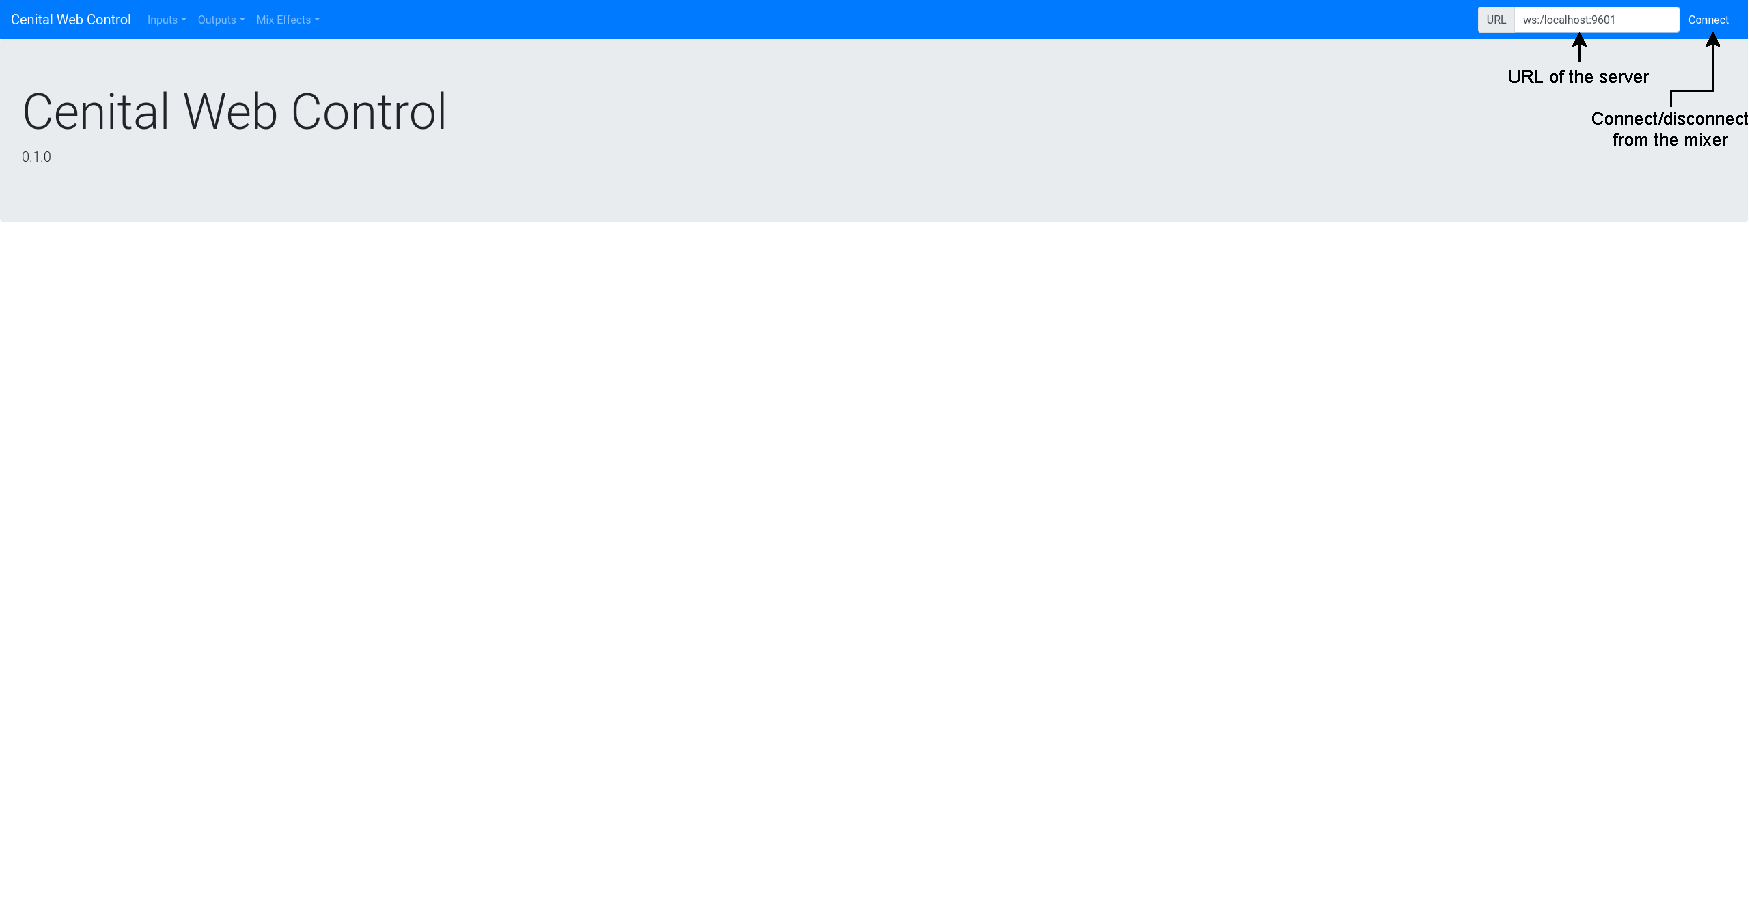
\includegraphics[width=\linewidth]{Home}
        \caption{Home page}
        \label{fig:home}
\end{figure}
\end{landscape}

\begin{landscape}
\begin{figure}[htbp]
        \centering
        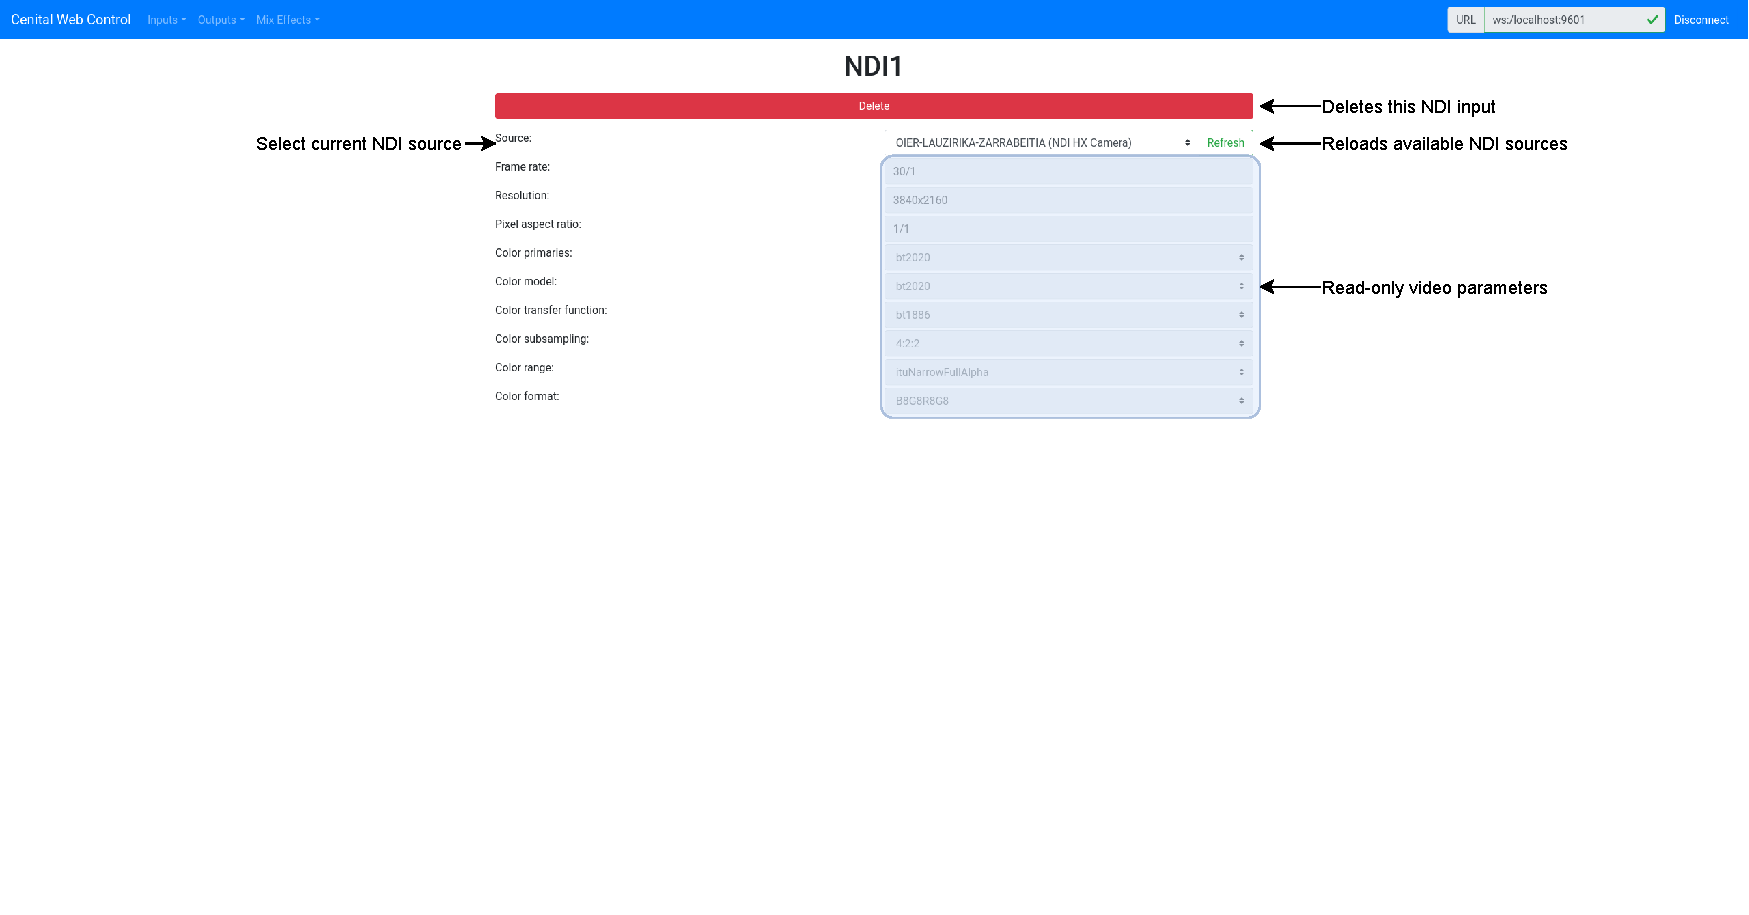
\includegraphics[width=\linewidth]{NDI}
        \caption{NDI input settings}
        \label{fig:ndi_input_settings}
\end{figure}
\end{landscape}


\begin{landscape}
\begin{figure}[htbp]
        \centering
        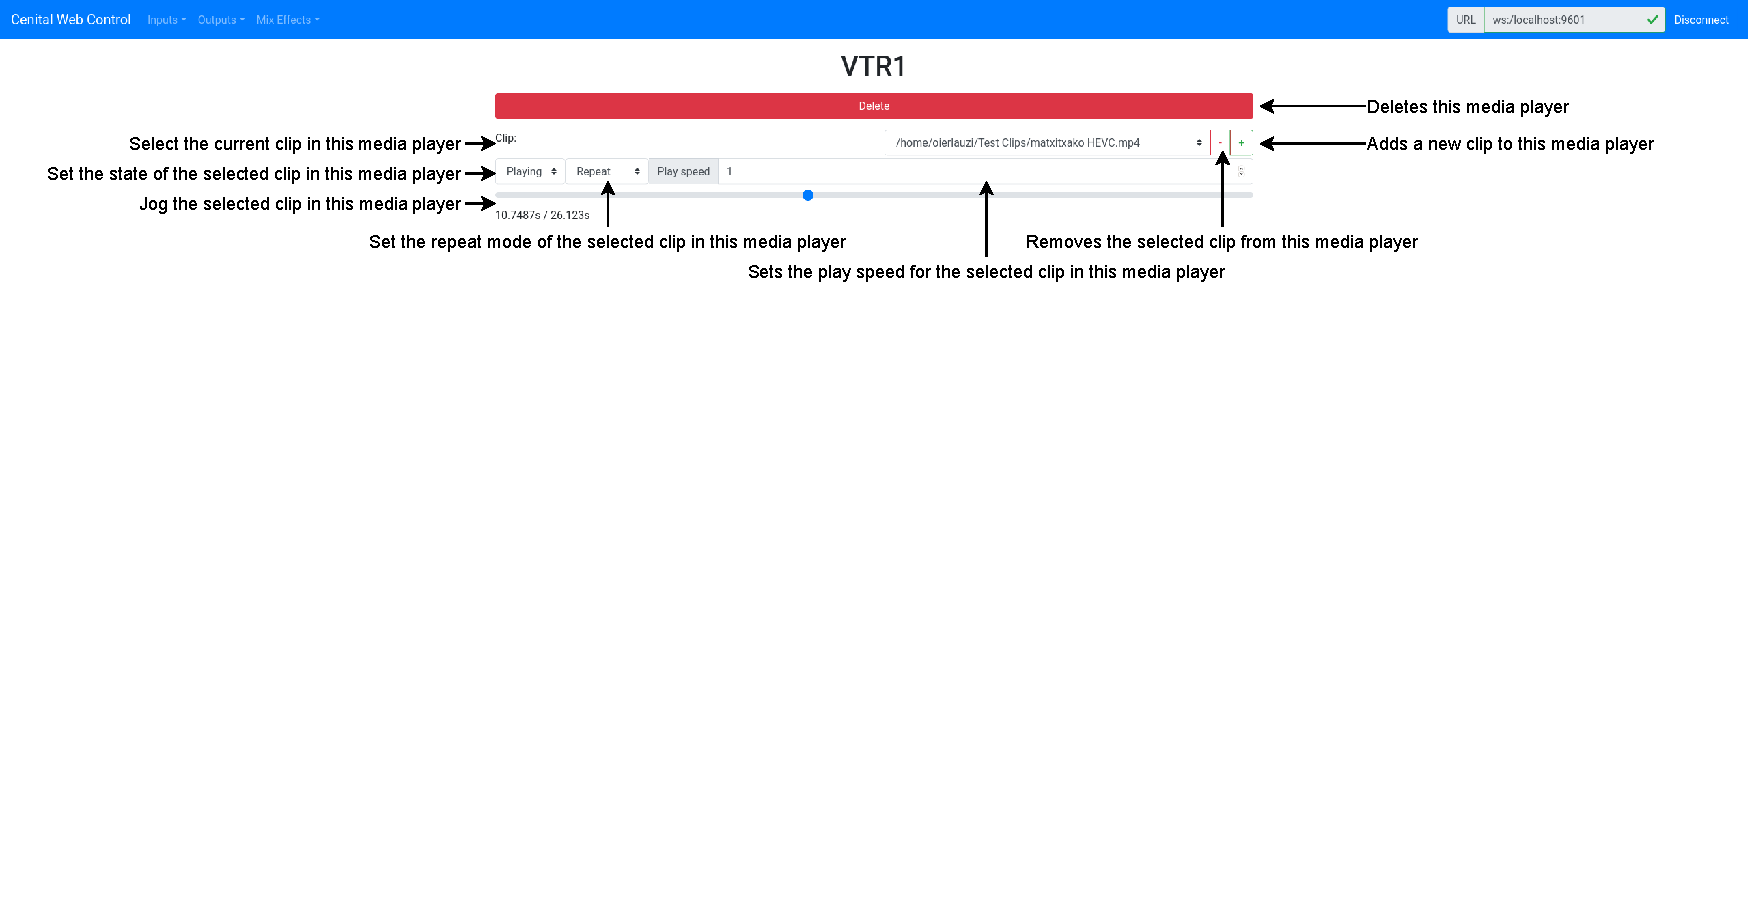
\includegraphics[width=\linewidth]{Media player}
        \caption{Media player settings}
        \label{fig:media_player_settings}
\end{figure}
\end{landscape}

\begin{landscape}
\begin{figure}[htbp]
        \centering
        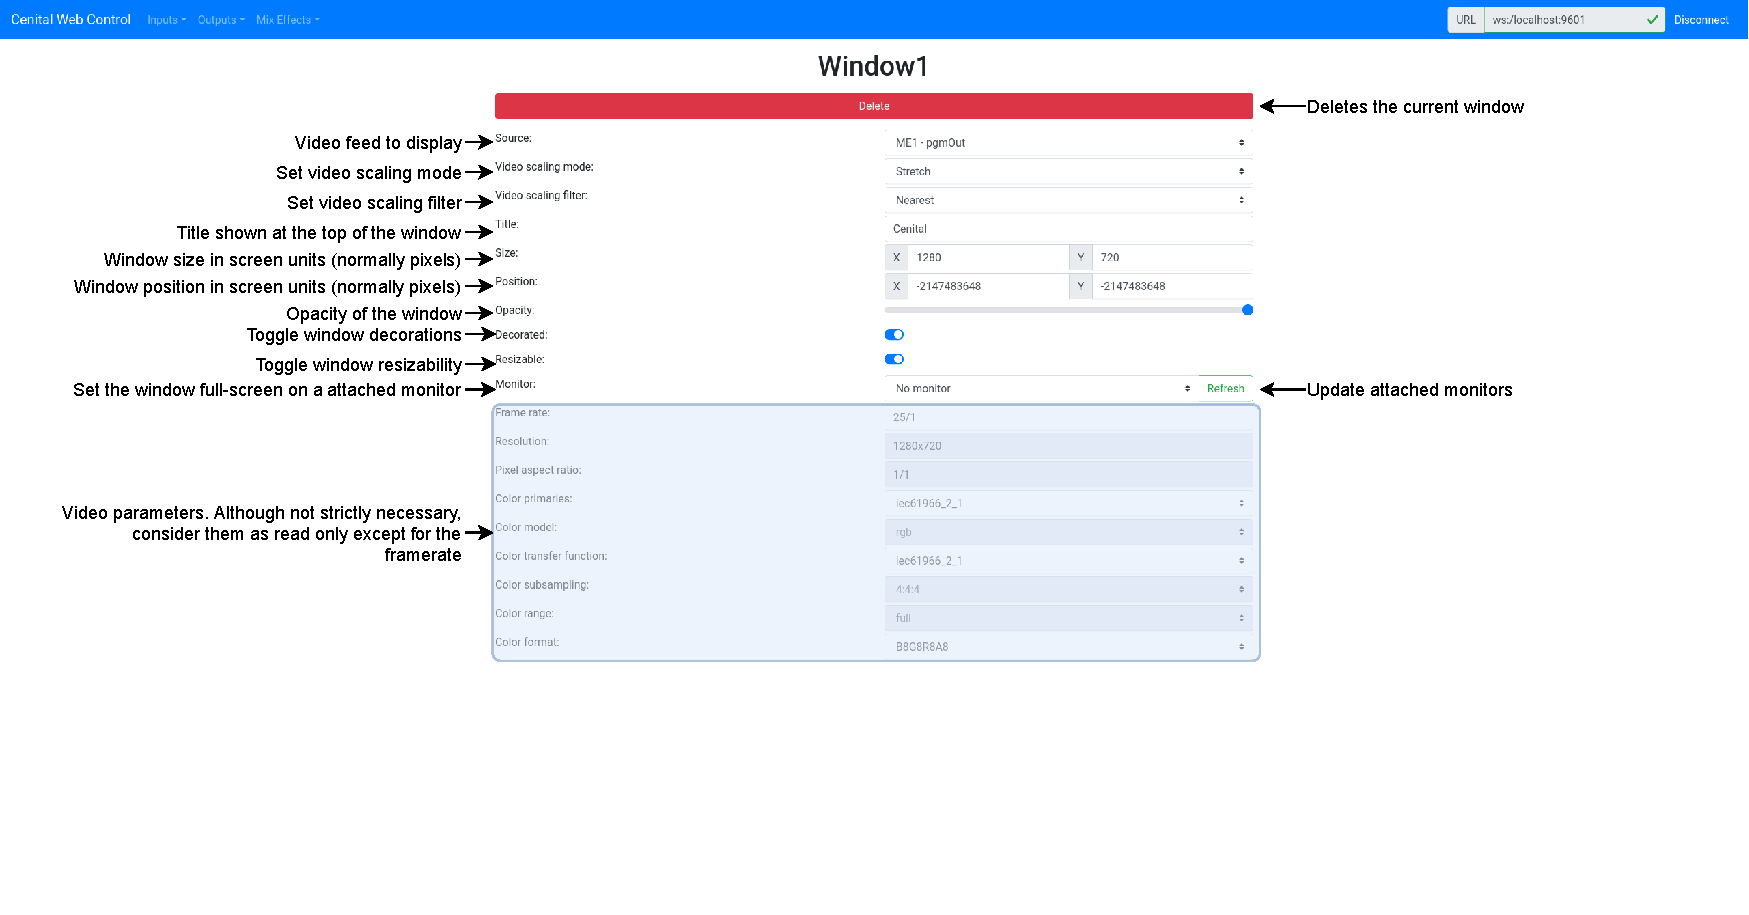
\includegraphics[width=\linewidth]{Window}
        \caption{Output window settings}
        \label{fig:output_window_settings}
\end{figure}
\end{landscape}



\begin{landscape}
\begin{figure}[htbp]
        \centering
        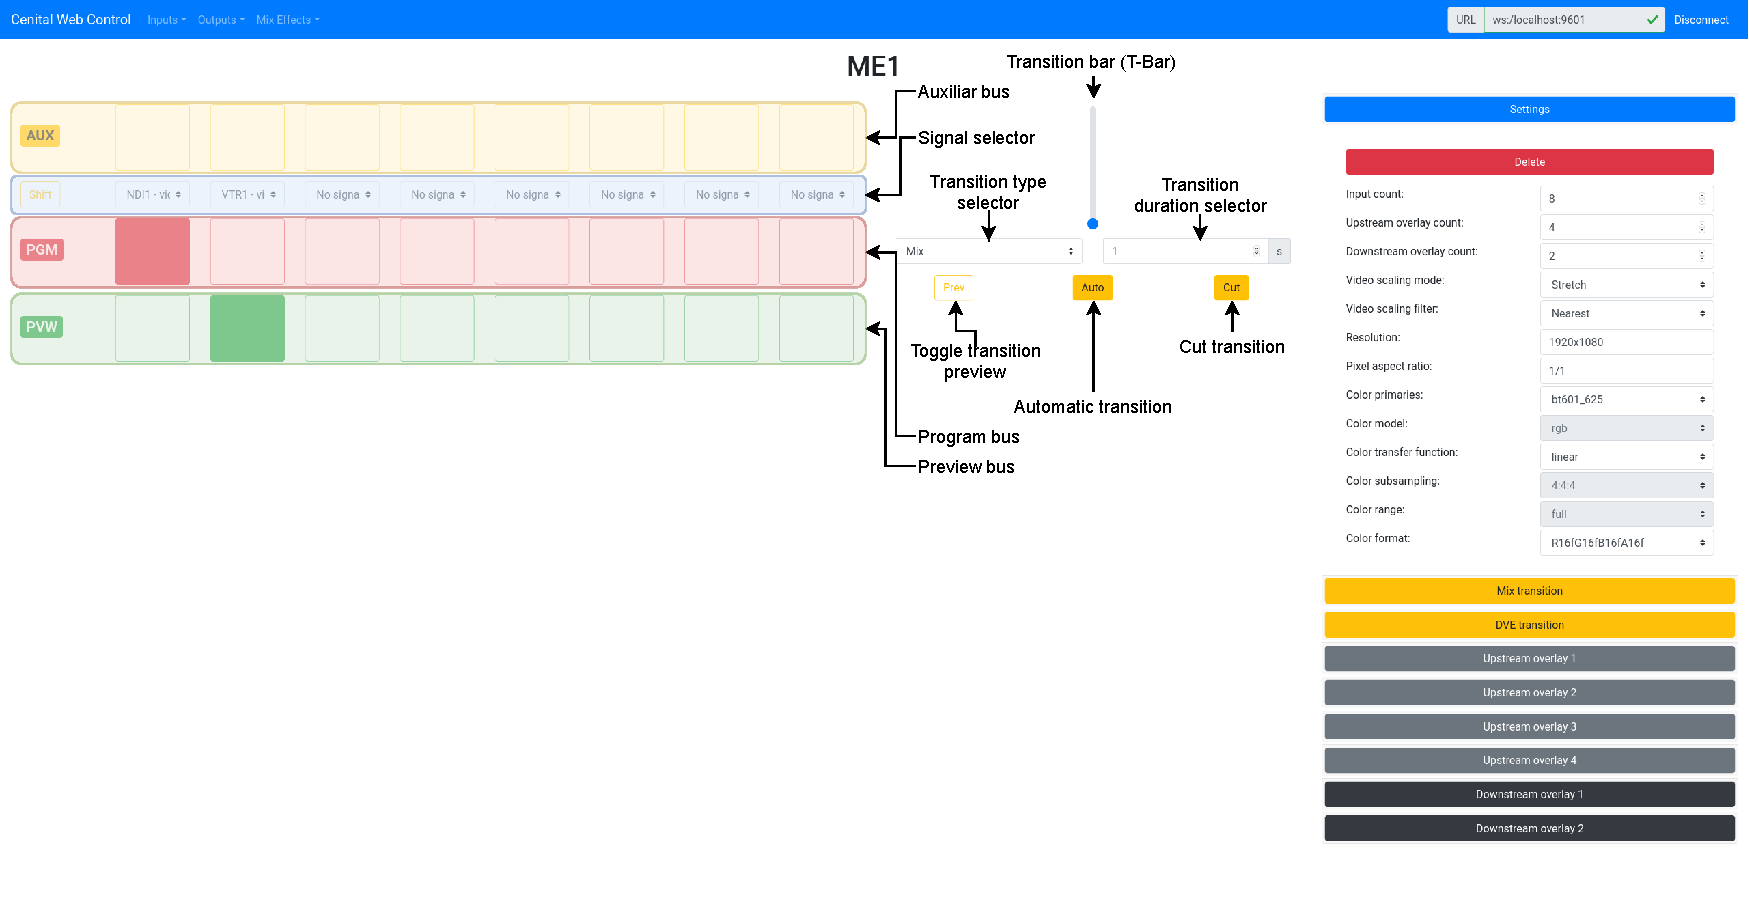
\includegraphics[width=\linewidth]{Mix effect}
        \caption{Crosspoint settings}
        \label{fig:mix_effect}
\end{figure}
\end{landscape}

\begin{figure}[htbp]
        \centering
        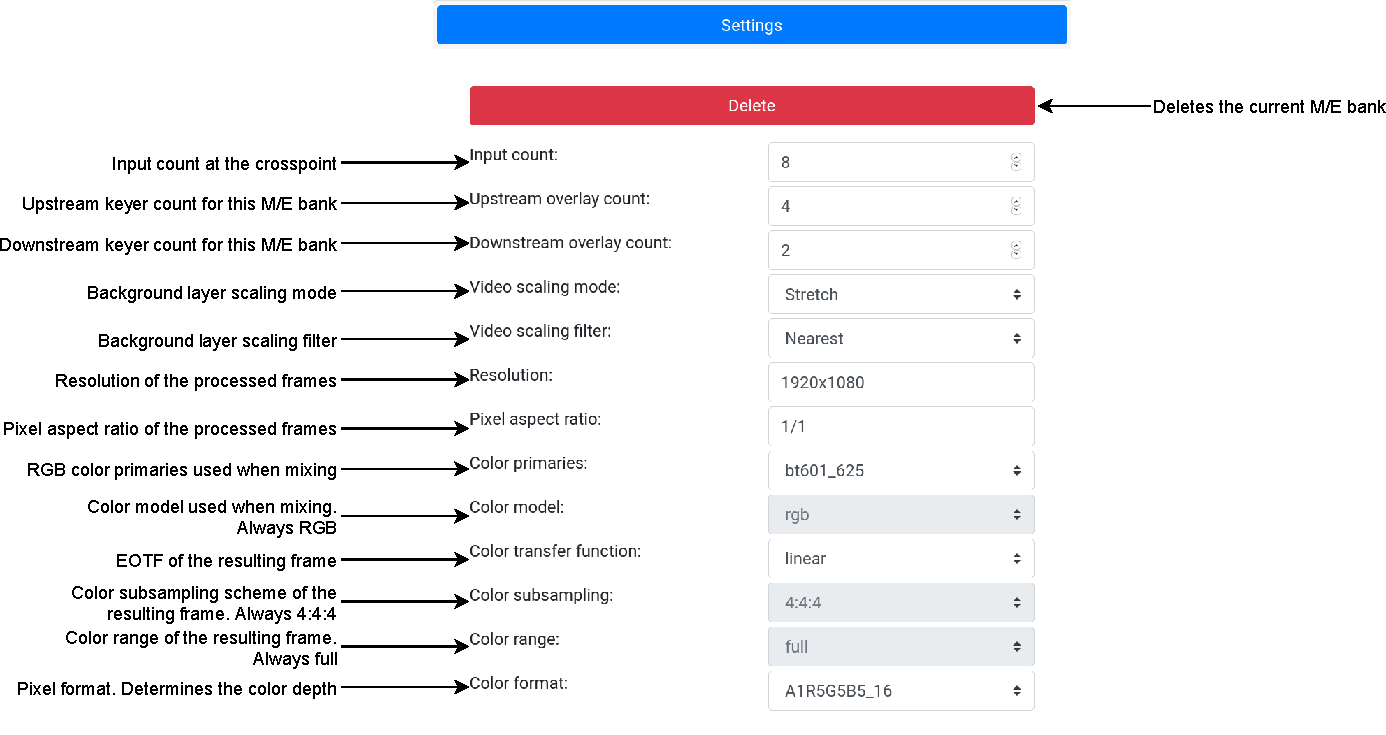
\includegraphics[width=\textwidth]{Mix effect settings}
        \caption{Mix effect settings}
        \label{fig:mix_effect_settings}
\end{figure}

\begin{figure}[htbp]
        \centering
        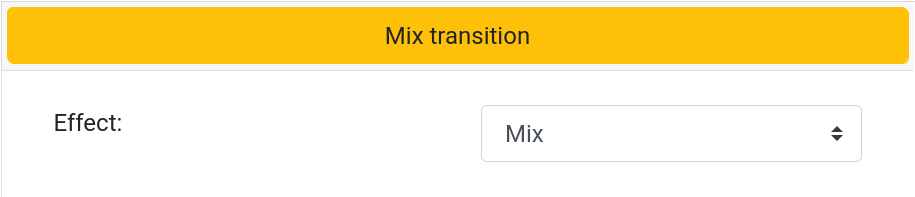
\includegraphics[width=.5\textwidth]{Transition-Mix}
        \caption{Mix transition settings}
        \label{fig:mix_effect_mix}
\end{figure}

\begin{figure}[htbp]
        \centering
        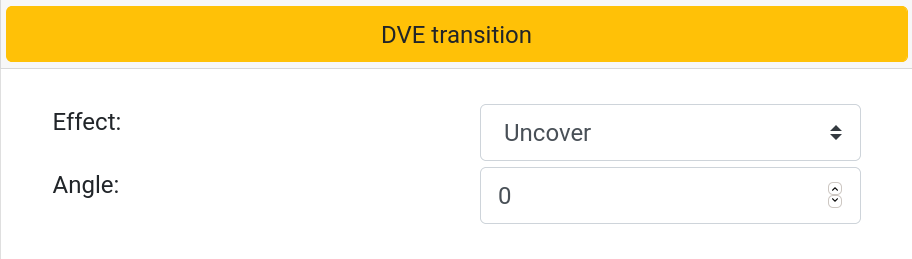
\includegraphics[width=.5\textwidth]{Transition-DVE}
        \caption{DVE transition settings}
        \label{fig:mix_effect_dve}
\end{figure}

\begin{figure}[htbp]
        \centering
        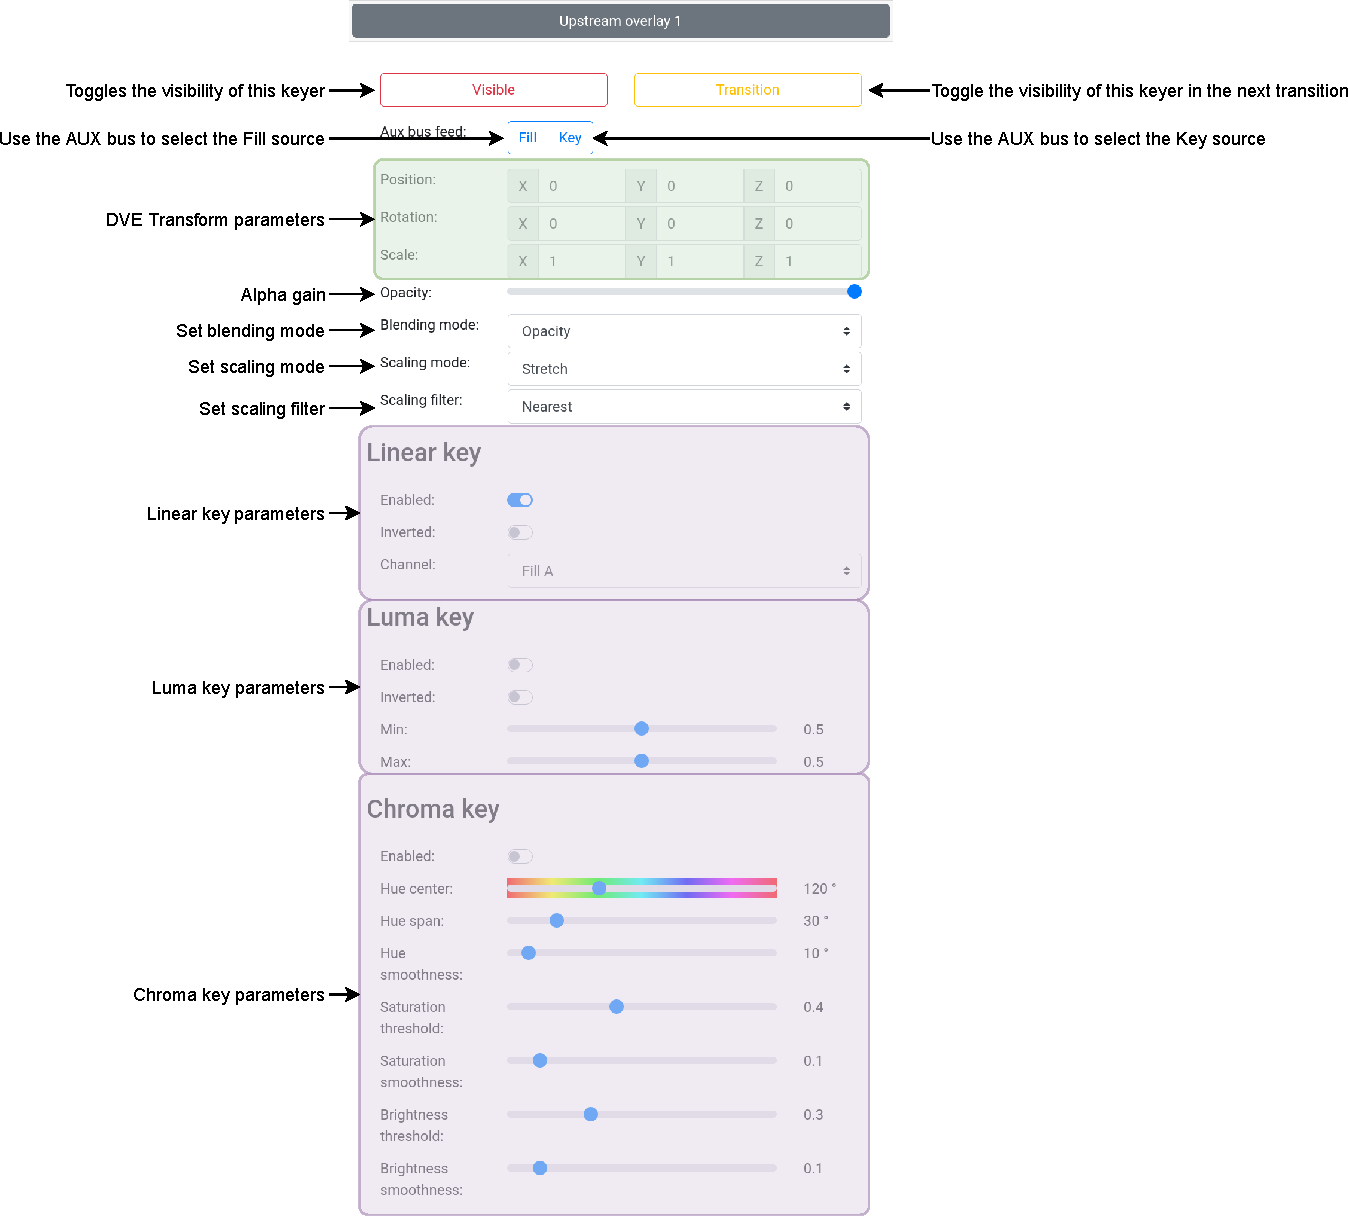
\includegraphics[width=\textwidth]{Keyer}
        \caption{Keyer settings}
        \label{fig:mix_effect_keyer}
\end{figure}

\end{document}
